\subsection{leftover}
what we would like to have is
\begin{align*}
    \E\left[D_{F^\star}\left(F'(a), F'(a) - \eta \hl\right)\right]
                        & \simeq
    \E\left[\left(
        \langle A, \ell \rangle
        -
        \E[
            \langle A, \ell \rangle | A
        ]
    \right)^2\right]\,. & (\text{what about }a?)
\end{align*}
\begin{center}
    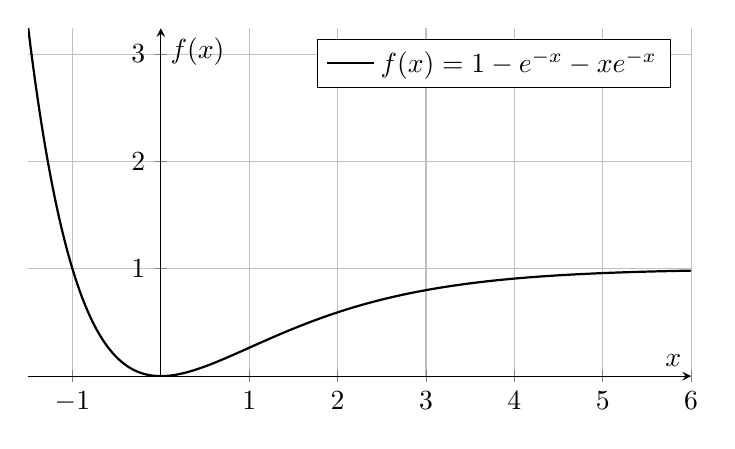
\begin{tikzpicture}
        \begin{axis}[
                width=10cm,
                height=6cm,
                axis lines=middle,
                xlabel={$x$},
                ylabel={$f(x)$},
                grid=both,
                domain=-1.5:6,
                samples=300,
                legend pos=north east,
            ]
            \addplot[thick] {1 - exp(-x) - x*exp(-x)};
            \addlegendentry{$f(x)=1-e^{-x}-x e^{-x}$};
        \end{axis}
    \end{tikzpicture}
\end{center}
\paragraph{The function \texorpdfstring{$f(x) = 1 - \exp(-x) - x \exp(-x)$}{f(x) = 1 - exp(-x) - x exp(-x)} and \texorpdfstring{$X \geq 0$}{X >= 0} a.s.}
Can we show that
\begin{align*}
    \E[f(X)] \simeq \E[X^2]\,?
\end{align*}

First, we have
\begin{align*}
    \E[X^2] = 2 \int_{0}^{\infty} t \PP(X \geq t) dt\,.
\end{align*}
Secondly, note that $f'(x) = x \exp(-x)$, and $f(0) = 0$. Hence,
$f(x) = \int_{0}^x t \exp(-t) dt$, so
\begin{align*}
    \E[f(X)]
    = \E\left[
        \int_0^X t \exp(-t) dt
        \right]
    = \int_0^\infty t \exp(-t) \PP(X \geq t) dt\,.
\end{align*}
Now, since $\exp(-t) \leq 1$ for $t \geq 0$, we have
\begin{align*}
    \E[f(X)] \leq \frac{\E[X^2]}{2}\,,
\end{align*}

However, if $X \in [0, B]$ a.s., then
\begin{align*}
    \E[f(X)]
     & = \int_0^\infty t \exp(-t) \PP(X \geq t) dt                                  \\
     & \geq \int_0^\infty t \exp(-B) \PP(X \geq t) dt                               \\
     & = \exp(-B)  \int_0^\infty t \PP(X \geq t) dt = \exp(-B) \frac{\E[X^2]}{2}\,.
\end{align*}

Given that $\E[f(X)] \geq \Var[X]$, (dropping $\exp(-B)$ for now) we have
\begin{align*}
    \E[f(-\eta \hl)|A]
     & \simeq \E[(-\eta \hl - \E[-\eta \hl|A])^2|A]                                             \\
     & =\E[(\eta Y \tfrac{T_A}{\eta P_A} - \E[\eta Y \tfrac{T_A}{\eta P_A}|A])^2|A]             \\
     & =( \tfrac{T_A}{ P_A})^2 \E[(Y - \E[Y|A])^2|A]                                            \\
     & =(\tfrac{T_A}{P_A})^2 \E[(\langle A, \ell\rangle - \E[\langle A, \ell\rangle|A])^2|A]\,,
\end{align*}
and putting back into eq~\ref{eq:linearized-D_F} gives
\begin{align*}
    D_{F^\star}\left(F'(a), F'(a) - \eta \hl\right)
     & =
    \langle a,
    1
    - \exp(-\eta \hl)
    - \eta \hl \odot \exp(-\eta \hl)
    \rangle
    \\
     & =
    (\tfrac{T_A}{P_A})^2 \langle a, \E[(\langle A, \ell\rangle - \E[\langle A, \ell\rangle|A])^2|A]
    \rangle\,,
\end{align*}
and further
\begin{align*}
    \E\left[D_{F^\star}\left(F'(a), F'(a) - \eta \hl\right)\right]
     & =
    \E\left[
        (\tfrac{T_A}{P_A})^2 \langle a, \E[(\langle A, \ell\rangle - \E[\langle A, \ell\rangle|A])^2|A]\rangle
    \right] \\
     & =
    \E\left[
        (\tfrac{T_A}{P_A})^2 \langle a, (\langle A, \ell\rangle - \E[\langle A, \ell\rangle|A])^2\rangle
        \right]
    \,,
\end{align*}




\clearpage
\paragraph{A Heavier Bayesian Approach}
Recall the original regret bound from theorem~\ref{thm:SMD-biased}
The expected regret of Biased-\smdalg is bounded by
\begin{align*}
    \Reg_n(a_\star) \leq
    \frac{D_F(a_\star, a_1)}{\eta} +
    \sum_{t=1}^{n}
    \E\left[
        \langle A_t - a_\star, \ell_t\rangle
        - \langle \fmd(\hl_{1:t-1}) - a_\star, \hl_t\rangle
        + \frac{1}{\eta} D_F(\fmd(\hl_{1:t-1}), \tfmd(\hl_{1:t}))
        \right]\,,
\end{align*}
and let's focus on the sum term.
The {\expbyopt}'s regret w.r.t. some $(a_\star, \ell_{1:n})$ is
\begin{align*}
     & \E\left[
        \sum_{t=1}^{n}
        \langle A_t - a_\star, \ell_t\rangle
        - \langle \fmd(\hl_{1:t-1}) - a_\star, \hl_t\rangle
        + \frac{1}{\eta} D_F(\fmd(\hl_{1:t-1}), \tfmd(\hl_{1:t}))
        \right]
    \\
     & =
    \E\left[
        \sum_{t=1}^{n}
        \min_{P_t, E_t}
        \E\left[
            \langle A_t - a_\star, \ell_t\rangle
            - \langle \fmd(\hl_{1:t-1}) - a_\star, \hl_t\rangle
            + \frac{1}{\eta} D_F(\fmd(\hl_{1:t-1}), \tfmd(\hl_{1:t}))
            | \fmd(\hl_{1:t-1})
            \right]
        \right]
    \\
     & =
    \min_{P_{1:n}, E_{1:n}}
    \E\left[
        \sum_{t=1}^{n}
        \E\left[
            \langle A_t - a_\star, \ell_t\rangle
            - \langle \fmd(\hl_{1:t-1}) - a_\star, \hl_t\rangle
            + \frac{1}{\eta} D_F(\fmd(\hl_{1:t-1}), \tfmd(\hl_{1:t}))
            | \fmd(\hl_{1:t-1})
            \right]
        \right]\,,
\end{align*}
so its minimax regret is bounded by
\begin{align*}
     & \min_{P_{1:n}, E_{1:n}}
    \sup_{(a_\star, \ell_{1:n}) \in \cA \times \cL^n}
    \E\left[
        \sum_{t=1}^{n}
        \E\left[
            \langle A_t - a_\star, \ell_t\rangle
            - \langle \fmd(\hl_{1:t-1}) - a_\star, \hl_t\rangle
            + \frac{1}{\eta} D_F(\fmd(\hl_{1:t-1}), \tfmd(\hl_{1:t}))
            | \fmd(\hl_{1:t-1})
            \right]
    \right]                    \\
     & \abovelabel{??} =
    \sup_{\nu \in \cP(\cA \times \cL^n)}
    \min_{P_{1:n}, E_{1:n}}
    \E\left[
        \sum_{t=1}^{n}
        \E\left[
            \langle A_t - A_\star, \ell_t\rangle
            - \langle \fmd(\hl_{1:t-1}) - A_\star, \hl_t\rangle
            + \frac{1}{\eta} D_F(\fmd(\hl_{1:t-1}), \tfmd(\hl_{1:t}))
            | \fmd(\hl_{1:t-1})
            \right]
    \right]                    \\
     & =
    \sup_{\nu \in \cP(\cA \times \cL^n)}
    \E\left[
        \sum_{t=1}^{n}
        \min_{P_t, E_t}
        \E\left[
            \langle A_t - A_\star, \ell_t\rangle
            - \langle \fmd(\hl_{1:t-1}) - A_\star, \hl_t\rangle
            + \frac{1}{\eta} D_F(\fmd(\hl_{1:t-1}), \tfmd(\hl_{1:t}))
            | \fmd(\hl_{1:t-1})
            \right]
    \right]                    \\
     & =
    \sup_{\nu \in \cP(\cA \times \cL^n)}
    \E\left[
        \sum_{t=1}^{n}
        \min_{P_t, E_t}
        \E\left[
            \langle A_t - A_\star, \ell_t\rangle
            - \langle \fmd(\hl_{1:t-1}) - A_\star, \hl_t\rangle
            + \frac{1}{\eta} D_F(\fmd(\hl_{1:t-1}), \tfmd(\hl_{1:t}))
            | A_{1:t-1}, Y_{1:t-1}
            \right]
    \right]                    \\
     & =
    \sup_{\nu \in \cP(\cA \times \cL^n)}
    \E\left[
        \sum_{t=1}^{n}
        \min_{P_t}
        \E\left[
            \langle A_t - A_\star, \ell_t\rangle
            -
            \frac{1}{\eta} D_F(\tfmd(\hl_{1:t}), \fmd(\hl_{1:t-1}))
            | A_{1:t-1}, Y_{1:t-1}
            \right]
    \right]                    \\
\end{align*}





\clearpage
\subsection{Bayesian setting, TS \& OSMD}
\textcolor{red}{TODO: rewrite  this section.}
\begin{algorithm}[h!]
    \begin{minipage}{12cm}
        \begin{mdframed}
            \begin{lstlisting}
args: $P$, $\eta$, $F$ and $E$ 
$\bar{A}_1 = \argmin_{a \in \cA} F(a)$
for $t = 1$ to $n$:
    Play $A_t \sim P_{A^b_t}$.
    Update $\bar{A}_{t+1} = \argmin_{a \in \cA} \eta \langle E(\bar{A}_t, A_t, Y_t), a \rangle + D_F(a, \bar{A}_t)$.
\end{lstlisting}
            \caption{OSMD}\label{alg:OSMD}
        \end{mdframed}
    \end{minipage}
\end{algorithm}
\citet{zimmert2019connections} suppose that (with simplifications)
\begin{enumerate}
    \item The exploration is done through a collection
          $P = \{P_a: a \in \cA\}$ such that $P_a \in \Delta(\cA)$ and
          $\E_{A \sim P_a}[A] = a$.
    \item The estimation is done through a function
          $E: \cA \times \cA \times \R \to \R^d$ such that
          \begin{align*}
              \E_{A \sim P_a}\left[
                  E(a, A, \underbrace{\langle \ell_t, A\rangle}_{Y_t})
                  \right] = \ell_t\,.
          \end{align*}
    \item Let $\texttt{MD}(\ell, b; \eta) = \argmin_{a \in \cA} \eta \langle \ell, a \rangle + D_F(a, b)$.
\end{enumerate}
The stability term is what inside the
expectation in Theorem~\ref{thm:SMD},
\begin{align*}
    \texttt{stab}_t(a) & \triangleq
    \E_{A_t \sim P_a}\left[
        \langle
        \hl_t,
        a - \bar{A}_{t+1}
        \rangle
        - \frac{D_F(\bar{A}_{t+1}, a)}{\eta}
        \right]
    \\
                       & =
    \E_{A_t \sim P_a}\left[
        \langle E(a, A_t, Y_t), a - \bar{A}_{t+1} \rangle
        - \frac{D_F(\bar{A}_{t+1}, a)}{\eta}
        \right]\,,
\end{align*}
where $\bar{A}_{t+1} = \texttt{MD}(\hl_t, \bar{A}_t)$,
which means the loss comes from $A_t$ but the `anchor' comes from $\bar{A}_t$.

\paragraph{Bayesian:}
Suppose that $(\ell_1, \ell_2, \cdots, \ell_n) \sim \nu$,
and $A_\star = \argmin_{a \in \cA} \sum_{t=1}^{n} \langle \ell_t, a\rangle$ is random.
The \textsf{MTS} \textit{Bayesian} algorithm just does one thing differently:
\begin{align*}
    \bar{A}^b_{t+1} = \E_{t}[A_\star]\,,
\end{align*}
so instead of \textsf{MD} update, it uses the expected optimal action.

The crucial connection is made through the fact that
\begin{align*}
    \E_{t-1}[A_t] = \E_{t-1}[A_\star]\,.
\end{align*}


\begin{algorithm}[h!]
    \begin{minipage}{8cm}
        \begin{mdframed}
            \begin{lstlisting}
args: Prior $\nu$, and $P$
$A_1^b = \E[A_\star]$
for $t = 1$ to $n$:
    Play $A_t \sim P_{A^b_t}$.
    Update $\bar{A}^b_{t+1} = \E_{t}[A_\star]$.
\end{lstlisting}
            \caption{MTS}\label{alg:MTS}
        \end{mdframed}
    \end{minipage}
\end{algorithm}

Beginning with the definition of the per-step Bayesian regret,
\begin{align*}
    \E_{t-1}[\Delta_t]
     & =\E_{t-1}[\langle A_t - A_\star, \ell_t \rangle]                 \\
     & =\E_{t-1}[\langle \bar{A}^b_t - A_\star, \hl_t \rangle]          \\
     & = \E_{t-1}[\langle \bar{A}^b_t - \bar{A}^b_{t+1}, \hl_t \rangle]
\end{align*}
Let $A_t \sim P_{\bar{A}^b_t}$, and recall the $\textsf{MD}$ update
\begin{align*}
    \texttt{MD}_t \triangleq \texttt{MD}(\hl_t, \bar{A}^b_t) = \argmin_{a \in \cA} \eta \langle \underbrace{E(\bar{A}^b_t, A_t, Y_t)}_{\hl_t}, a \rangle + D_F(a, \bar{A}^b_t)\,,
\end{align*}
so
\begin{align*}
     & \langle \hl_t, \texttt{MD}_t \rangle + \frac{1}{\eta} D_F(\texttt{MD}_t, \bar{A}_t^b)
    \leq
    \langle \hl_t, \bar{A}^b_{t+1} \rangle + \frac{1}{\eta}D_F(\bar{A}^b_{t+1}, \bar{A}_t^b)                 \\
    \Rightarrow
     & \langle \hl_t, \texttt{MD}_t - \bar{A}_{t}^b \rangle + \frac{1}{\eta} D_F(\texttt{MD}_t, \bar{A}_t^b)
    \leq
    \langle \hl_t, \bar{A}^b_{t+1} - \bar{A}_{t}^b \rangle + \frac{1}{\eta}D_F(\bar{A}^b_{t+1}, \bar{A}_t^b) \\
    \Rightarrow
     & \langle \hl_t, \bar{A}_{t}^b - \bar{A}^b_{t+1} \rangle
    \leq
    \langle \hl_t, \bar{A}_{t}^b - \texttt{MD}_t \rangle
    +
    \frac{1}{\eta}D_F(\bar{A}^b_{t+1}, \bar{A}_t^b)
    - \frac{1}{\eta} D_F(\texttt{MD}_t, \bar{A}_t^b)\,,
\end{align*}
which gives
\begin{align*}
    \E_{t-1}[\Delta_t]
     & = \E_{t-1}[\langle \bar{A}^b_t - \bar{A}^b_{t+1}, \hl_t \rangle] \\
     & \leq \E_{t-1}\left[
    \underbrace{
        \langle \hl_t, \bar{A}_{t}^b - \texttt{MD}_t \rangle
        - \frac{1}{\eta} D_F(\texttt{MD}_t, \bar{A}_t^b)}_{
        \texttt{stab}_t(\bar{A}_t^b; \eta)
    }
    +\frac{1}{\eta}D_F(\bar{A}^b_{t+1}, \bar{A}_t^b)
    \right]                                          \,,                \\
\end{align*}
which means bounding the $\texttt{stab}_t(a, \eta)$ gives a regret bound for the Bayesian regret
since the sum of divergences is bounded by \citet{lattimore2019information}[Thm 3].

\section{Bandit convex optimization(\bco)}
The losses sequence is a sequence of convex functions
$f_1, f_2, \cdots, f_n: \cA \to \R$.
In each round $t$, the learner chooses an action $A_t \in \cA$,
and observes $Y_t = f_t(A_t) \in \R$.
\subsection{\bco in one dimension}
Suppose that $\cA = [-1, 1]$.
We use the idea of covering + \mdalg on simplex as discussed in
section~\ref{sec:md-negentropy} to solve this setting.

Let $\cC_\epsilon = \{ \alpha\epsilon: \alpha \in \mathbb{Z}, \alpha\epsilon \in [-1, 1]\}$ be an $\epsilon$-covering of $\cA$.
Let
\begin{align*}
    \ell_t =
    \begin{bmatrix}
        f_t(c_1) \\
        f_t(c_2) \\
        \vdots   \\
        f_t(c_n)
    \end{bmatrix}\,, \quad \text{where } c_i \in \cC_\epsilon\,,
\end{align*}
and with that the 1D \bco problem is reduced (with $n\epsilon$ looseness
due to covering) to a \blo problem in $d=\ceil{2/\epsilon}$ dimensions,
with the action space $\cA_\blo = \Delta(\ceil{2/\epsilon})$.

\begin{remark}[\textcolor{red}{$n^{3/4}$} upper-bound for \textit{Lip}-Bandits]
    Naively applying the bound on \mdalg with $\epsilon=\frac{1}{\sqrt{n}}$
    from remark~\ref{rem:md-simplex-explicit} gives an upper-bound of
    $\sqrt{2 n \cdot d} = \sqrt{2 n \cdot \ceil{2/\epsilon}}= n^{3/4}$
    on the \blo reduction, which together with the covering
    error of $\sqrt{n}$ results in a bound of $\tilde{O}(n^{3/4})$.
    This applies to all Lipschitz bandits.
\end{remark}

The main idea to get $\widetilde{O}(\sqrt{n})$ bound is to exploit
the fact that not all $\ell \in [0,1]^d$ are possible in the
\blo-reduction: $\ell_t$ is a discretization of a
convex function.
The result should be a better bound on the sum in
theorem~\ref{thm:md-simplex}.

\begin{remark}[Actions are distributions when $\cA=\Delta(d)$]\label{rem:actions-are-dists}
    The very nice (and weird) thing about running any algorithm
    on the simplex with linear losses is that if it plays $A_t \in \Delta(\cA)$,
    which could be random itself, it can be further
    restricted to play $e_{\omega}$ with $\omega \sim A_t$, without
    changing the \textit{conditional expected per step loss}.
    With that in mind, \mdalg does come with a default randomization
    in the simplex: instead of playing $\fmd(\ell_{1:t-1})$
    play $e_\omega$ with $\omega \sim \fmd(\ell_{1:t-1})$.
\end{remark}

\paragraph{Randomness in the virtual game}
The algorithm knows the estimates $\hl_{1:t-1}$,
so it's technically in the \olo setting in the virtual game,
where it can simply run \mdalg \textbf{with no randomness}---just
take $\hat{a}_t = \fmd(\hl_{1:t-1})$.
However, everything is unchanged if the algorithm
decides to randomize in the \textit{virtual game}.
The algorithm can play a distribution $Q_t \in \Delta(\cC)$
with $\E_{A \sim Q_t}[A] = \hat{a}_t$.
The benefit of this will be clear in a moment.

To emphasize the fact that $\hat{a}_t$ is a distribution
we use $Q_t\triangleq \hat{a}_t$ to be the \textit{virtual policy}:
\begin{align*}
    Q_t(\omega) & = \hat{a}_t^\top e_\omega\,, \forall \omega \in \cC\,,
\end{align*}
and let $K \in \R^{|\cC| \times |\cC|}$ be a probability kernel,
meaning that $K Q_t \in \Delta(\cC)$.
Then we choose $P_t \in \Delta(\cC)$ to be
\begin{align*}
    P_t & = K Q_t\,,
\end{align*}
and note that $A_t \sim P_t$ can be written as
\begin{align*}
    A_t = e_{\alpha_t}\,, \qquad \text{where } \alpha_t \sim P_t\,.
\end{align*}


\paragraph{A chance to make Biased-\smdalg somewhat unbiased:}
So far $\E_t[A_t] \neq \fmd(\hl_{1:t-1})$
necessarily, but we can choose $P_t$
such that they are \textit{jointly} unbiased:
\begin{align*}
    \langle \ell_t, P_t \rangle
     & =
    \E_t\left[\langle \hl_t, e_{\beta_t}\rangle\right]
    =
    \langle \E[\hl_t], Q_t \rangle\,,
\end{align*}
where $\beta_t \sim Q_t$ is the virtual action.
This can be done by setting
\begin{align*}
    \hl_t & = E(e_{\alpha_t}, Y_t)
    = E(e_{\beta_t}, \langle \alpha_t, \ell_t\rangle)
    = \frac{K^\top e_{\alpha_t} \cdot \langle e_{\alpha_t}, \ell_t\rangle}{
        P_t^\top e_{\alpha_t}
    }\,,
\end{align*}
since then
\begin{align*}
    \E_t\left[\hl_t\right]
     & =
    \E_t\left[
        \frac{K^\top e_{\alpha_t} \cdot \langle e_{\alpha_t}, \ell_t\rangle}{
            P_t^\top e_{\alpha_t}}
    \right] \\
     & =
    \sum_{\alpha \in \cC}
    \frac{K^\top e_{\alpha}
        \cdot \langle e_{\alpha}, \ell_t\rangle}{
        P_t^\top e_{\alpha}}
    P_t^\top e_{\alpha}
    \\
     & =
    \sum_{\alpha \in \cC}
    K^\top e_{\alpha}
    \cdot \langle e_{\alpha}, \ell_t\rangle
    \\
     & =
    K^\top \ell_t\,,
\end{align*}
and finally
\begin{align*}
    \langle \ell_t, P_t \rangle
    = \langle \ell_t, K Q_t \rangle
    = \langle K^\top \ell_t, Q_t \rangle
    = \langle \E_t[\hl_t], Q_t \rangle\,.
\end{align*}

\paragraph{A specific choice of \texorpdfstring{$K$}{K}---exploiting 1d geometry:}
Let $\bar{A}$ be
\begin{align*}
    \bar{A}_t = \langle P_t, \cC \rangle,
\end{align*}
which should be thought of as the expected action in round $t$.
Let $\Pi_\cC(x) = \argmin_{y \in \cC, |y| \leq |x|} |x - y|$,
Given $I(x,y) = \{z \in \cC: \min(x,y) \leq z \leq \max(x,y)\}$,
let
\begin{align*}
    K_{x,y} & =
    \begin{cases}
        \frac{1}{|I(x,y)|} & \text{if } x\in I(\bar{A}_t, y) \\
        0                  & \text{otherwise}
    \end{cases}\,,
\end{align*}

\begin{lemma}[\cite{lattimore2024bandit}[Lemma 8.3]]
    We have
    \begin{align*}
        \langle \ell_t, P_t - e_{b} \rangle
        \leq 2 \cdot \langle \E_t[\hl_t], Q_t - e_{b} \rangle\,,
    \end{align*}
    and
    \begin{align*}
        \E_t[(e_{\beta_t}^\top \hl_t)^2]
        \leq 2 + \ln(n)
    \end{align*}
\end{lemma}

\hrulefill
\section{Negentropy potential}

\section{Closed form for \texorpdfstring{$\cA = [d]$}{A = [d]}?}
Let's look back at the result of Lemma~\ref{lem:E-optimized-Lambda}:
\begin{align*}
    \Lambda(P, E_{T^\star} || \nu)
     & =
    \E\!\left[
        \frac{1}{\eta}
        \langle A - A_\star, \ell\rangle
        -
        \frac{1}{\eta^2}
        D_{F^\star}\left(F'(a), F'(a) - \eta \hl\right)
        \right]\,.
\end{align*}
Two questions arise for $\cA = [d]$, and $F$ being the negentropy:
\begin{itemize}
    \item What does $\Lambda(P, E_{T^\star} || \nu)$ look like?
    \item Can we have a closed form for $T^\star$?
\end{itemize}
Note that an action $A \sim P$ is simply $A = e_a$ with probability $P_a$.
Therefore, there is no policy optimization, since for a given $P \in \Delta(d)$,
there is only one set of weights $P_a$ such that
\begin{align*}
    P = \sum_{a=1}^d P_a e_a\,,
\end{align*}
which means that once the learner chooses $E_{T^\star}$, the value of the game is determined.

For the first question, we have
\begin{align}
    D_{F^\star}\left(F'(a), F'(a) - \eta \hl\right)
     & =
    F^\star(F'(a)) - F^\star(F'(a) - \eta \hl)
    - \eta {F^\star}'(F'(a) - \eta \hl) \hl
    \nonumber
    \\
     & =
    \langle 1, a\rangle -
    \langle 1, a \odot \exp(-\eta \hl)\rangle
    -
    \langle 1, a \odot \exp(-\eta \hl) \odot \eta \hl\rangle
    \nonumber
    \\
     & =
    \langle a,
    1
    - \exp(-\eta \hl)
    - \eta \hl \odot \exp(-\eta \hl)
    \rangle
    \label{eq:linearized-D_F}
    \\
     & =
    \langle a,
    1
    - \exp(-Y \tfrac{T_A}{\eta P_A})
    - Y \tfrac{T_A}{\eta P_A} \odot \exp(-Y \tfrac{T_A}{\eta P_A})
    \rangle\,.\nonumber
\end{align}
For the second question, we should look at \cref{thm:optimal-mult-y} and
see if we can solve for $T^\star$ in closed form.
Starting from the result of \cref{thm:optimal-mult-y} we have
\begin{align*}
    \E\!\left[
        Y A_\star
        | A = b
        \right]
     & =
    \E\!\left[
        Y {F^\star}'\left(F'(a) - \tfrac{Y}{P_b}T_b\right)
        | A = b
    \right] \nonumber \\
    \abovelabel{F negentropy}
    \Rightarrow
    \E\!\left[
        Y A_\star
        | A = b
        \right]
     & =
    \E\!\left[
        Y \exp\left(\ln(a) - \tfrac{Y}{\eta P_b}T_b\right)
        | A = b
    \right] \nonumber \\
     & =
    a \odot
    \E\!\left[
        Y \exp\left(- \tfrac{Y}{\eta P_b}T_b\right)
        | A = b
    \right] \nonumber \\
    \abovelabel{$Y = \langle \ell, b\rangle$, and $A \perp \ell, A_\star$}
    \Rightarrow
    \E\!\left[
        \ip{\ell, b} A_\star
        \right]
     & =
    a \odot
    \E\!\left[
        \ip{\ell, b} \exp\left(- \tfrac{\ip{\ell, b}}{\eta P_b}T_b\right)
        \right]
    \\
    \abovelabel{$b$ is one-hot}
    \Rightarrow
    \E\!\left[
        \ell_b A_\star
        \right]
     & =
    a \odot
    \E\!\left[
        \ell_b \exp\left(- \tfrac{\ell_b}{\eta P_b}T_b\right)
        \right]
    \\
    \abovelabel{$z$-th coord}
    \Rightarrow
    \E\!\left[
        \ell_b A_{\star, z}
        \right]
     & =
    a_z \cdot
    \E\!\left[
        \ell_b \exp\left(- \tfrac{\ell_b}{\eta P_b}T_{b, z}\right)
        \right]
    \\
     & =
    a_z \cdot
    \E\!\left[
        \ell_b
        \exp\left(- \tfrac{T_{b, z}}{\eta P_b}\ell_b\right)
        \right]
    \\
     & =
    a_z \cdot
    M_{\ell_{b}}'\left(- \tfrac{T_{b, z}}{\eta P_b}\right)
\end{align*}
Therefore, since the inverse of $M_{\ell_b}'$ is well-defined,
and is bijective from $(-\infty, \infty)$ to $(0, \infty)$,
we have
\begin{align*}
    T_{b, z}
     & =
    - \eta P_b
    {M_{\ell_b}'}^{-1}\left(
    \frac{\E\!\left[
        \ell_b A_{\star, z}
        \right]}{a_z}
    \right)\,.
\end{align*}

\clearpage
\paragraph{The problem with linear loss class}
Consider the \olo problem over $\cK = [-1, 1]$.
For a discretization dimension $d$
and a real number $m_\ell$, define the loss
\begin{align*}
    \ell = (-m_\ell, -\tfrac{d-1}{d}m_\ell, \cdots,
    -\tfrac{1}{d}m_\ell, 0, \tfrac{1}{d}m_\ell,
    \tfrac{2}{d}m_\ell, \cdots, \tfrac{d-1}{d} m_\ell, m_\ell),
\end{align*}
and the action set is the simplex $\Delta(2d + 1)$.

Then for an action $p \in \Delta(2d + 1)$ we have
\begin{align*}
    \langle \ell, p\rangle = m_\ell
    \langle
    (-1, -\tfrac{d-1}{d}, \cdots, -\tfrac{1}{d},
    0, \tfrac{1}{d}, \cdots, \tfrac{d-1}{d}, 1)
    , p
    \rangle\,,
\end{align*}
which means the \textit{effective action} is
$
    A \triangleq
    \langle
    (-1, -\tfrac{d-1}{d}, \cdots, -\tfrac{1}{d},
    0, \tfrac{1}{d}, \cdots, \tfrac{d-1}{d}, 1)
    , p
    \rangle
    \in [-1, 1]
$ and
\begin{align*}
    Y = \langle p, \ell \rangle = m_\ell A,\,\,
    \text{and}
    \qquad
    \hl = Y \tfrac{T_A}{P_A} = m_\ell A \tfrac{T_A}{P_A}\,.
\end{align*}
Then Thm~\ref{thm:optimal-mult-y} translates to
\begin{align*}
    \E\!\left[
        \hl \odot A_\star
        | A
        \right]
     & =
    \E\!\left[
        \hl \odot {F^\star}'\left(F'(a) - \eta \hl\right)
        | A
        \right]
    \\
    \Rightarrow
    \E\!\left[
        m_\ell A \tfrac{T_A}{P_A} \odot A_\star
        | A
        \right]
     & =
    \E\!\left[
        m_\ell A \tfrac{T_A}{P_A} \odot {F^\star}'\left(F'(a) - \eta m_\ell A \tfrac{T_A}{P_A}\right)
        | A
        \right]
    \\
    \abovelabel{$A,T_A \neq 0$}
    \Rightarrow
    \E\!\left[
        m_\ell \odot A_\star
        | A
        \right]
     & =
    \E\!\left[
        m_\ell \odot {F^\star}'\left(F'(a) - \eta m_\ell A \tfrac{T_A}{P_A}\right)
        | A
        \right]
    \\
    \abovelabel{$F$ negentropy}
    \Rightarrow
    \E\!\left[
        m_\ell \odot A_\star
        | A
        \right]
     & =
    \E\!\left[
        m_\ell \odot \exp\left(\ln(a) - \eta m_\ell A \tfrac{T_A}{P_A}\right)
        | A
        \right]
    \\
    \Rightarrow
    \E\!\left[
        m_\ell \odot A_\star
        | A
        \right]
     & =
    a \odot
    \E\!\left[
        m_\ell \odot \exp\left(- \eta m_\ell A \tfrac{T_A}{P_A}\right)
        | A
        \right]
    \\
    \abovelabel{For each coord $z$}
    \Rightarrow
    \E\!\left[
        m_\ell \odot A_\star
        | A
        \right]
     & =
    a_z
    \E\!\left[
        m_\ell \odot \exp\left(- \eta m_\ell A \tfrac{T_{A,z}}{P_A}\right)
        | A
        \right]\,,
\end{align*}
Now if the LHS is negative, there's no solution for $T_{A,z}$.

\paragraph{The linear \& positive loss class}
Consider the \olo problem over $\cK = [0, 1]$.
For a discretization dimension $d$
and real numbers $m_\ell, b_\ell$, define the loss
\begin{align*}
    \ell = (-m_\ell, -\tfrac{d-1}{d}m_\ell, \cdots,
    -\tfrac{1}{d}m_\ell, 0, \tfrac{1}{d}m_\ell, \cdots,
    \tfrac{d-1}{d} m_\ell, m_\ell) + b_\ell,
\end{align*}
and the action set is the simplex $\Delta(2d + 1)$.

Then for an action $p \in \Delta(2d + 1)$ we have
\begin{align*}
    \langle \ell, p\rangle = m_\ell
    \langle
    (-1, -\tfrac{d-1}{d}, \cdots, -\tfrac{1}{d},
    0, \tfrac{1}{d}, \cdots, \tfrac{d-1}{d}, 1)
    , p
    \rangle + b_\ell\,,
\end{align*}
which means the \textit{effective action} is
$
    A \triangleq
    \langle
    (-1, -\tfrac{d-1}{d}, \cdots, -\tfrac{1}{d},
    0, \tfrac{1}{d}, \cdots, \tfrac{d-1}{d}, 1)
    , p
    \rangle
    \in [-1, 1]
$ and
\begin{align*}
    Y = \langle p, \ell \rangle = m_\ell A + b_\ell,\,\,
    \text{and}
    \qquad
    \hl = Y \tfrac{T_A}{P_A} = (m_\ell A + b_\ell) \tfrac{T_A}{P_A}\,,
\end{align*}
\textbf{and it's guaranteed that $Y=m_\ell A + b_\ell \geq 0$}.
Then Thm~\ref{thm:optimal-mult-y} translates to
\begin{align*}
    \E\!\left[
        \hl \odot A_\star
        | A
        \right]
     & =
    \E\!\left[
        \hl \odot {F^\star}'\left(F'(a) - \eta \hl\right)
        | A
        \right]
    \\
    \Rightarrow
    \E\!\left[
        (m_\ell A + b_\ell) \tfrac{T_A}{P_A} \odot A_\star
        | A
        \right]
     & =
    \E\!\left[
        (m_\ell A + b_\ell) \tfrac{T_A}{P_A} \odot {F^\star}'\left(F'(a) - \eta (m_\ell A + b_\ell) \tfrac{T_A}{P_A}\right)
        | A
        \right]
    \\
    \abovelabel{$A,T_A \neq 0$}
    \Rightarrow
    \E\!\left[
        (m_\ell A + b_\ell) \odot A_\star
        | A
        \right]
     & =
    \E\!\left[
        (m_\ell A + b_\ell) \odot {F^\star}'\left(F'(a) - \eta (m_\ell A + b_\ell) \tfrac{T_A}{P_A}\right)
        | A
        \right]
    \\
    \abovelabel{$F$ negentropy}
    \Rightarrow
    \E\!\left[
        (m_\ell A + b_\ell) \odot A_\star
        | A
        \right]
     & =
    \E\!\left[
        (m_\ell A + b_\ell) \odot \exp\left(\ln(a) - \eta (m_\ell A + b_\ell) \tfrac{T_A}{P_A}\right)
        | A
        \right]
    \\
    \Rightarrow
    \E\!\left[
        (m_\ell A + b_\ell) \odot A_\star
        | A
        \right]
     & =
    a \odot
    \E\!\left[
        (m_\ell A + b_\ell) \odot \exp\left(- \eta m_\ell A \tfrac{T_A}{P_A}\right)
        | A
        \right]
    \\
    \abovelabel{For each coord $z$}
    \Rightarrow
    \E\!\left[
        (m_\ell A + b_\ell) \odot A_\star
        | A
        \right]
     & =
    a_z
    \E\!\left[
        (m_\ell A + b_\ell) \odot \exp\left(- \eta (m_\ell A + b_\ell) \tfrac{T_{A,z}}{P_A}\right)
        | A
        \right]\,,
\end{align*}
Now, there's always a solution for $T_{A,z}$.